\section{Price endogeneity and instruments}\label{sec:07-endogeneity}

The Berry inversion turns logit demand into a linear equation. With market shares observed in markets
$t = 1, \dots, T$, \cref{eq:07-logit-inversion} reads
\begin{equation}\label{eq:07-est-eq}
  y_{jt} \equiv \ln s_{jt} - \ln s_{0t} = x_{jt}\beta - \alpha p_{jt} + \xi_{jt}.
\end{equation}
The left side is data. The right side contains the observed characteristics $x_{jt}$, the price $p_{jt}$ and the
unobserved product characteristic $\xi_{jt}$, which now plays the role of a regression error. Equation
\eqref{eq:07-est-eq} looks like a textbook regression, and it is tempting to estimate it by ordinary least squares
(OLS). This section explains why OLS fails, which instruments the literature uses instead, what each instrument
assumes, and what instrumenting does in practice. It closes with a Monte Carlo experiment that replicates the one in
\citet{Berry1994}.

\subsection{Why prices are endogenous}\label{sec:07-endog-bias}

Prices are chosen by firms, and firms know $\xi_{jt}$. The unobserved characteristic stands for everything that
consumers value and the econometrician does not measure. Examples are the styling and perceived quality of a car, the
reputation of a brand, the effect of past advertising, a favorable shelf position, or the quality of after-sales
service. Each of these raises demand. A firm that faces higher demand for its product sets a higher price. So the
price and the error in \eqref{eq:07-est-eq} move together.

The logit model makes this link explicit. Suppose each firm sells one product, marginal cost $mc_{jt}$ is constant, and
firms set prices in a Nash equilibrium. \Cref{sec:07-supply} shows that the equilibrium price is
\begin{equation}\label{eq:07-price-decomp}
  p_{jt} = mc_{jt} + m_{jt}, \qquad m_{jt} = \frac{1}{\alpha(1 - s_{jt})},
\end{equation}
where $m_{jt}$ is the dollar markup (\cref{prop:07-logit-markup}). The markup depends on $\xi_{jt}$ through the share.
To see the size of the effect, hold rivals' prices and the marginal cost fixed and raise $\xi_j$ by $\dd\xi$ (we drop
the market index). The share changes because $\delta_j$ rises by $\dd\xi$ and falls by $\alpha\,\dd m_j$. With the
derivatives of \cref{prop:07-logit-derivs},
\begin{equation*}
  \dd s_j = s_j(1 - s_j)\,(\dd\xi - \alpha\,\dd m_j).
\end{equation*}
Differentiating the markup in \eqref{eq:07-price-decomp} gives $\dd m_j = \frac{\dd s_j}{\alpha(1 - s_j)^2} = \alpha
m_j^2\,\dd s_j$. Substituting the first expression into the second,
\begin{align*}
  \dd m_j &= \alpha m_j^2 s_j (1 - s_j)\,(\dd\xi - \alpha\,\dd m_j) \\
          &= m_j s_j\,(\dd\xi - \alpha\,\dd m_j),
\end{align*}
where the second line uses $\alpha m_j (1 - s_j) = 1$. Collecting the terms in $\dd m_j$,
\begin{equation*}
  \dd m_j\,(1 + \alpha m_j s_j) = m_j s_j\,\dd\xi .
\end{equation*}
Since $1 + \alpha m_j s_j = 1 + \frac{s_j}{1 - s_j} = \frac{1}{1 - s_j}$, we obtain
\begin{equation}\label{eq:07-dp-dxi}
  \frac{\partial p_j}{\partial \xi_j} = \frac{\partial m_j}{\partial \xi_j} = m_j s_j (1 - s_j) = \frac{s_j}{\alpha} > 0 .
\end{equation}
A product with a higher unobserved quality therefore carries a higher price even when its cost does not depend on
quality. If better quality is also more expensive to produce, so that $mc_{jt}$ rises with $\xi_{jt}$, the cost channel
adds to the markup channel. In both cases $\Cov(p_{jt}, \xi_{jt}) > 0$.

\citet[p.~320]{Nevo2001} writes the same argument in general form. Any Nash pricing rule gives $p_{jt} = mc_{jt} +
f(\xi_{jt}, \dots)$. Decompose the marginal cost and the markup into a product mean and a market-specific deviation,
\begin{equation}\label{eq:07-nevo-decomp}
  p_{jt} = (mc_j + f_j) + (\Delta mc_{jt} + \Delta f_{jt}).
\end{equation}
Both components of the markup depend on the corresponding components of $\xi_{jt}$. The mean component is the
persistent quality of a brand, and the deviation is a local or temporary demand shock that firms observe and react to.
Fixed effects deal with the first (\cref{sec:07-fixed-effects}). Instruments must deal with the second.

The consequence for OLS is the familiar omitted-variable bias. The next proposition states it for
\eqref{eq:07-est-eq} and also gives the bias in the taste coefficients, which is less often written down.

\begin{proposition}[OLS bias in the logit regression]\label{prop:07-ols-bias}
Let the observations $(j, t)$ be such that sample second moments converge to their population counterparts. Suppose
\eqref{eq:07-est-eq} holds with $\E[\xi_{jt}] = 0$ and $\E[x_{jt}^\top \xi_{jt}] = 0$, where $x_{jt}$ contains a
constant. Let $p_{jt} = x_{jt}\Gamma + \tilde p_{jt}$ be the linear projection of price on $x_{jt}$, with residual
$\tilde p_{jt}$ and $\Var(\tilde p_{jt}) > 0$. Define
\begin{equation*}
  b = \frac{\Cov(p_{jt}, \xi_{jt})}{\Var(\tilde p_{jt})}.
\end{equation*}
Then the OLS estimates from the regression of $y_{jt}$ on $(x_{jt}, p_{jt})$ satisfy
\begin{equation}\label{eq:07-ols-bias}
  \plim \hat\alpha_{OLS} = \alpha - b, \qquad \plim \hat\beta_{OLS} = \beta - \Gamma b .
\end{equation}
If $\Cov(p_{jt}, \xi_{jt}) > 0$, then $\hat\alpha_{OLS}$ is biased toward zero, and it converges to a negative number
(an upward-sloping demand curve) when $\Cov(p_{jt}, \xi_{jt}) > \alpha\Var(\tilde p_{jt})$.
\end{proposition}

\begin{proof}
OLS converges to the coefficients of the linear projection of $y_{jt}$ on $(x_{jt}, p_{jt})$. We compute that
projection in three steps. First, substitute $p_{jt} = x_{jt}\Gamma + \tilde p_{jt}$ into \eqref{eq:07-est-eq}:
\begin{equation*}
  y_{jt} = x_{jt}(\beta - \alpha\Gamma) - \alpha\tilde p_{jt} + \xi_{jt}.
\end{equation*}
Second, project $\xi_{jt}$ on $(x_{jt}, \tilde p_{jt})$. By construction $\E[x_{jt}^\top\tilde p_{jt}] = 0$, so the
two regressors are orthogonal and each coefficient is a simple regression coefficient. The coefficient on $x_{jt}$ is
zero because $\E[x_{jt}^\top\xi_{jt}] = 0$. The coefficient on $\tilde p_{jt}$ is
\begin{equation*}
  \frac{\E[\tilde p_{jt}\xi_{jt}]}{\E[\tilde p_{jt}^2]} = \frac{\E[p_{jt}\xi_{jt}] - \Gamma^\top\E[x_{jt}^\top
  \xi_{jt}]}{\Var(\tilde p_{jt})} = \frac{\Cov(p_{jt}, \xi_{jt})}{\Var(\tilde p_{jt})} = b,
\end{equation*}
where we used $\E[\tilde p_{jt}] = 0$ and $\E[\xi_{jt}] = 0$, which hold because $x_{jt}$ contains a constant. Hence
the projection of $y_{jt}$ on $(x_{jt}, \tilde p_{jt})$ is $x_{jt}(\beta - \alpha\Gamma) + (b - \alpha)\tilde p_{jt}$.
Third, substitute back $\tilde p_{jt} = p_{jt} - x_{jt}\Gamma$:
\begin{align*}
  x_{jt}(\beta - \alpha\Gamma) + (b - \alpha)(p_{jt} - x_{jt}\Gamma)
  &= x_{jt}\bigl(\beta - \alpha\Gamma - (b - \alpha)\Gamma\bigr) + (b - \alpha)p_{jt} \\
  &= x_{jt}(\beta - \Gamma b) - (\alpha - b)p_{jt}.
\end{align*}
The coefficient on $p_{jt}$ is $-(\alpha - b)$, so $\plim\hat\alpha_{OLS} = \alpha - b$. The coefficient on $x_{jt}$
is $\beta - \Gamma b$. The last two claims follow because $b > 0$ when the covariance is positive, and $\alpha - b < 0$
exactly when $\Cov(p_{jt}, \xi_{jt}) > \alpha\Var(\tilde p_{jt})$.
\end{proof}

OLS therefore makes demand look too inelastic. It also biases downward the coefficient of any characteristic that
raises price ($\Gamma_k > 0$), because it attributes to price part of what the characteristic is worth.
\Cref{sec:07-montecarlo} confirms both predictions numerically.

The bias has a sharp economic signature. A profit-maximizing firm never prices on the inelastic part of its demand
curve, since a small price increase would then raise revenue and lower cost. Formally, \cref{prop:07-logit-multi}
below gives $p_j - mc_j = \frac{1}{\alpha(1 - S_f)}$ for a firm with combined share $S_f \geq s_j$. Since $mc_j > 0$,
\begin{equation}\label{eq:07-elastic-check}
  1 > \frac{p_j - mc_j}{p_j} = \frac{1}{\alpha p_j (1 - S_f)} \geq \frac{1}{\alpha p_j (1 - s_j)} = \frac{1}{\varepsilon_j},
\end{equation}
so the own-price elasticity $\varepsilon_j = \alpha p_j(1 - s_j)$ (\cref{sec:07-logit-elasticities}) exceeds one
under any ownership structure. Counting the products with $\hat\alpha p_j(1 - s_j) < 1$ is a cheap specification
check.

\subsection{Instruments}\label{sec:07-instruments}

The remedy is instrumental variables (IV). Let $z_{jt}$ be a row vector of $L$ instruments. It contains the $K$ exogenous
characteristics $x_{jt}$ and $L - K$ excluded variables.

\begin{assumption}[Instruments for the logit regression]\label{asm:07-iv}
\leavevmode
\begin{enumerate}[label=(\roman*)]
  \item \emph{Exogeneity.} The instruments satisfy $\E[\xi_{jt} \mid z_t] = 0$, where $z_t$ collects the instruments
    of all products in market $t$. The weaker unconditional version is $\E[z_{jt}^\top\xi_{jt}] = 0$.
  \item \emph{Relevance (rank).} The $L \times (K+1)$ matrix $\E[z_{jt}^\top (x_{jt}, p_{jt})]$ has full column rank
    $K + 1$. In particular, at least one excluded instrument must be correlated with $p_{jt}$ after partialling out
    $x_{jt}$.
\end{enumerate}
\end{assumption}

The conditional version of (i) is the assumption of \citet[eq.~4.1]{BerryLevinsohnPakes1995}. It implies that any
function of $z_t$ is a valid instrument, so the practical question is which functions to use. Prices and quantities
are excluded from $z_t$ because the model determines them jointly with $\xi$. Characteristics and cost shifters are
included because the model does not explain them, and that choice drives most of the debate below.

Three families of excluded instruments dominate the literature. We take them in turn and then discuss what fixed
effects add.

\casehead{Cost shifters}
A \emph{cost shifter} $w_{jt}$ moves marginal cost and does not enter utility. Examples are input prices (the price
of milk for yogurt), wages, exchange rates for imported goods, and taxes on producers. They are the traditional
instruments in homogeneous-goods markets, and \citet[p.~249]{Berry1994} notes that they ``continue to be
appropriate'' with differentiated products. Their validity rests on the independence of cost and demand shocks.

Cost shifters are scarce in practice. They must vary across products or markets in ways that fixed effects do not
absorb, and an input price common to all products is collinear with time effects.
\citet[pp.~161, 164]{HausmanLeonardZona1994} observe that at the brand level ``excluded cost shifting variables
\dots\ may be difficult to find.'' A characteristic that enters cost but not utility also works.
\citet[p.~874]{BerryLevinsohnPakes1995} put miles per gallon in cost and miles per dollar in utility, because the cost
of building a fuel-efficient car does not depend on the price of gasoline. The ideal instrument, a product-specific
cost shifter, is the hardest to find.

\casehead{Characteristics of other products}
\citet[p.~249]{Berry1994} pointed out a second source of exogenous price variation. In a model with exogenous
characteristics, ``the characteristics of other firms ($x_k$, $k \neq j$) are also appropriate instruments.'' They are
excluded from the utility of product $j$, and they are correlated with its price ``via the markups in the first-order
conditions.'' Berry calls this ``a specific example of the general proposition that, in imperfectly competitive markets,
demand-side instruments can be variables that affect markups as well as variables that affect marginal cost.'' A
product that faces close substitutes has a low markup. A product in an empty region of the characteristic space has a
high one.

\citet[Section~5.1]{BerryLevinsohnPakes1995}, BLP hereafter, turned the idea into the \emph{BLP instruments}. Their starting point is
the efficient instrument under a conditional moment restriction \citep{Chamberlain1987}. Take the logit regression with
parameters $\theta_1 = (\beta, \alpha)$, and suppose the errors are homoskedastic and uncorrelated across products. The
efficient instrument for observation $(j, t)$ is then
\begin{equation}\label{eq:07-optimal-iv}
  z^{*}_{jt} = \E\Bigl[\frac{\partial\xi_{jt}(\theta_1)}{\partial\theta_1} \Bigm| z_t\Bigr]
  = \bigl(-x_{jt},\; \E[p_{jt} \mid z_t]\bigr),
\end{equation}
since $\xi_{jt}(\theta_1) = y_{jt} - x_{jt}\beta + \alpha p_{jt}$. The efficient instrument for price is the expected
equilibrium price given all exogenous variables. Computing it requires solving the pricing game for many draws of the
unobservables, integrating over them, and selecting among equilibria \citep[p.~860]{BerryLevinsohnPakes1995}. A series
approximation in the characteristics of all $J_t$ products would need a number of terms that grows with $J_t$. BLP
avoid this with an exchangeability argument \citep{Pakes1994}. An equilibrium does not change when we reorder rival
firms, a rival's products, or a firm's other products. The first-order basis functions for characteristic $k$ of
product $j$, owned by firm $f$, are then
\begin{equation}\label{eq:07-blp-iv}
  x_{jkt}, \qquad z^{\mathrm{own}}_{jkt} = \sum_{r \in \mathcal{J}_f,\, r \neq j} x_{rkt}, \qquad
  z^{\mathrm{riv}}_{jkt} = \sum_{r \notin \mathcal{J}_f} x_{rkt}.
\end{equation}
With the constant among the characteristics, the numbers of own and rival products are instruments too. The sums vary
because they exclude product $j$, because firms own different sets of products, and because the product set changes
over time. BLP found higher-order terms nearly collinear with the linear ones. They use 15 demand-side instruments
(three terms for each of five demand characteristics) and 19 cost-side instruments
\citep[pp.~861--862]{BerryLevinsohnPakes1995}.

The logit model shows why the sums are relevant. Under multi-product pricing every product of firm $f$ carries the
markup $\frac{1}{\alpha(1 - S_f)}$ (\cref{prop:07-logit-multi}). The firm's combined share $S_f = \frac{\sum_{k \in
\mathcal{J}_f} e^{\delta_k}}{1 + \sum_{k} e^{\delta_k}}$ falls when rival products become more attractive and rises
when the firm adds products. So $z^{\mathrm{riv}}$ shifts the markup down and $z^{\mathrm{own}}$ shifts it up, holding
the product's own characteristics fixed. In richer models the markup depends on the distance to the nearest
competitors, which is why BLP separate own and rival sums.

The exogeneity of characteristics deserves scrutiny. It requires that characteristics be chosen without knowledge of
$\xi$, or independently of it. \citet[p.~854]{BerryLevinsohnPakes1995} acknowledge that if a ``true'' model jointly
determines observed and unobserved characteristics, their assumption ``will only be correct if that model has very
specific properties.'' A weaker alternative for panel data lets $\xi$ and $\omega$ follow a first-order Markov process
whose innovations are independent of a model's initial characteristics. BLP judged it ``much more demanding of the
data'' \citep[p.~855]{BerryLevinsohnPakes1995}.

Is it enough that characteristics are predetermined, that is, chosen before prices? It is not. Predetermination
concerns timing, while exogeneity concerns information. A manufacturer that knows its new model has attractive
styling may also give it more horsepower, because horsepower pays more in a car that sells well. Then $\E[\xi_{jt}
\mid x_t] \neq 0$ although $x_t$ was fixed long before prices were set. Timing delivers exogeneity only if $\xi_{jt}$
was unpredictable when $x_t$ was chosen, which is the Markov assumption above. \citet[p.~320]{Nevo2001} remarks that
treating characteristics as predetermined ``is as reasonable (or unreasonable)'' in his application ``as it was in
previous work.''

Characteristic-based instruments are therefore often called inefficient and probably inconsistent. They are
inefficient because the sums in \eqref{eq:07-blp-iv} are a linear approximation to $\E[p_{jt} \mid z_t]$, which is a
nonlinear function of all characteristics. Approximations to the efficient instrument evaluate the model's derivatives
at a preliminary estimate, with the unobservables set to their mean of zero. In Monte Carlo studies of the random
coefficients logit, \citet{ReynaertVerboven2014} find that such instruments reduce small-sample bias and are even
more effective at improving precision and stability. The characteristic-based instruments are probably inconsistent
because characteristics respond to demand. Most researchers recognize both problems and use these instruments for
lack of better ones.

A third problem appears in markets with many products. As the number of products grows, each logit share goes to
zero, and the markup $\frac{1}{\alpha(1 - s_j)}$ converges to the constant $\frac{1}{\alpha}$. The variation in prices
that rival characteristics induce then vanishes, and the instruments become weak. \citet{Armstrong2016} formalizes
this point with asymptotics in the number of products per market. He considers single-product firms and logit
demand, or random coefficients logit demand without a random coefficient on price. Markups then converge to
$\frac{1}{\alpha}$ so fast that estimates based on BLP instruments are inconsistent. Cost shifters escape the problem
because they move prices without moving markups. BLP instruments keep their power in other settings, for example
with logit demand and a fixed number of asymmetric multi-product firms.
Our Monte Carlo extension in \cref{tab:07-mc-weak} illustrates the point.

\emph{Differentiation instruments} \citep[Section~2.3]{GandhiHoude2019} refine the BLP idea.
Substitution depends on proximity in the characteristic space, so these instruments use the differences $d_{jrk} =
x_{rkt} - x_{jkt}$ between product $j$ and each other product $r$ in the market. The \emph{local} version counts rivals within a band,
$\sum_r \indic\{|d_{jrk}| < \kappa_k\}$, with $\kappa_k$ a proximity threshold, for example the standard deviation of
characteristic $k$ across markets. The \emph{quadratic} version is $\sum_r d_{jrk}^2$. Both share the exogeneity
assumption of the BLP sums. \citet[p.~7]{GandhiHoude2019} take excluded instruments for price as given. They design
differentiation instruments to identify the parameters that govern substitution in random coefficients demand
(\cref{ch:blp}).

\casehead{Prices in other markets (Hausman instruments)}
A third family uses panel data in which the same products are sold in many cities.
\citet[p.~164]{HausmanLeonardZona1994} model the log price of brand $j$ in city $n$ and period $\tau$ as
\begin{equation}\label{eq:07-hlz-price}
  \ln p_{jn\tau} = \delta_j \ln c_{j\tau} + \alpha_{jn} + \omega_{jn\tau} .
\end{equation}
Here $c_{j\tau}$ is a cost common to all cities, since the products are sold at a uniform national wholesale price.
The term $\alpha_{jn}$ is a city-brand effect for transport costs or local wages, and $\omega_{jn\tau}$ is a local
shock such as a promotion. (The symbols $\delta_j$ and $\alpha_{jn}$ are used only in this display.) Suppose the local
shocks are independent across cities. After brand and city effects, the price of $j$ in other cities then moves with
the common cost and is uncorrelated with the local demand shock. With a market $t$ defined as a city-period pair, the
\emph{Hausman instrument} is the average price of the same product in the set $\mathcal{N}_{-t}$ of other cities in the
same period,
\begin{equation}\label{eq:07-hausman-iv}
  \bar p_{j,-t} = \frac{1}{|\mathcal{N}_{-t}|} \sum_{t' \in \mathcal{N}_{-t}} p_{jt'} .
\end{equation}
\Cref{ch:aids} discusses its first use, and \citet{Hausman1997} applies it to cereal. \citet[pp.~320--321]{Nevo2001}
uses regional average prices of the brand in all twenty quarters, excluding the city being instrumented. He assumes
that, ``controlling for brand-specific means and demographics, city-specific valuations are independent across
cities.''

Hausman instruments fail when demand shocks are correlated across markets. A national advertising campaign raises
demand, and hence prices, in every city. Nevo's example is the discovery that fiber reduces the risk of cancer.
Promotions coordinated within a region break the assumption for nearby cities. \citet[p.~242]{Bresnahan1997} pressed
this objection against Hausman's cereal study. With nationwide demand shocks, he argues, the own-price coefficients are
``biased upward, toward zero,'' and the estimator ``is like doing ordinary least squares'' on a supply and demand
system. His appendix derives the asymptotic bias (pp.~246--247). Its sign and size depend on the covariance matrix of
the national component of the demand shock (p.~242). Hausman's assumption that this matrix is zero removes the bias.
Nevo focuses on established brands, absorbs aggregate shocks with time dummies, and compares the
results with a second instrument set. It consists of proxies for city-level marginal cost: region dummies, city
density and supermarket wages. Agreement between instruments with different threats is his main evidence. Hausman
instruments also require the same product in many markets, so they are unavailable for national markets like
automobiles.

\casehead{Endogenous characteristics and the long run}
Exogenous characteristics are also built into counterfactuals. A merger simulation or a tax analysis usually holds
the set of products and their characteristics fixed, which makes it a short-run exercise. In the long run firms
reposition their products. \citet{Sweeting2010} finds that firms that buy competing music radio stations
differentiate their playlists. \citet{Fan2013} shows that ignoring the adjustment of newspaper characteristics
``causes substantial differences in estimated effects of mergers'' (\cref{ch:mergers}). Once characteristics are
choices, characteristic-based instruments lose their justification and fixed-characteristic counterfactuals lose their
realism. Product-specific cost shifters solve only the first problem. \citet[p.~259]{Berry1994} already noted that a
full solution requires ``a reasonable model of the dynamic process that generates product characteristics.''

\subsection{Product and market fixed effects}\label{sec:07-fixed-effects}

Panel data allow a different treatment of the persistent part of $\xi$. Suppose the same products appear in many
markets, and write $\xi_{jt} = \bar\xi_j + \Delta\xi_{jt}$. Including a product fixed effect $d_j$ in
\eqref{eq:07-est-eq} gives
\begin{equation}\label{eq:07-fe-eq}
  y_{jt} = d_j + \lambda_t - \alpha p_{jt} + \Delta\xi_{jt}, \qquad d_j = x_j\beta + \bar\xi_j ,
\end{equation}
where $\lambda_t$ is a market or time effect and $x_j$ does not vary across markets. The product effect absorbs the
persistent quality $x_j\beta + \bar\xi_j$, the main source of correlation between prices and $\xi$ in cross sections.
\citet[p.~322]{Nevo2001} adds that brand dummies improve the fit when observed characteristics are incomplete, and that
the number of parameters grows with $J$, not $J^2$.

Fixed effects do not end the endogeneity problem. The remaining error $\Delta\xi_{jt}$ is the market-specific deviation
in \eqref{eq:07-nevo-decomp}, and firms price on it. Identification of $\alpha$ now comes from price variation within
a product across markets, which Hausman instruments and local cost shifters supply. BLP instruments do not if
characteristics and choice sets are fixed. With brand dummies in the regression, Nevo's characteristic-based
instrument matrix ``will be essentially singular'' \citep[p.~320]{Nevo2001}. Brand dummies can instead serve as
instruments, a nonparametric way to use all the information in fixed characteristics.

The taste parameters $\beta$ are recovered in a second step. Let $\hat d$ be the $J \times 1$ vector of estimated
product effects, $V_d$ its covariance matrix, and $X$ the $J \times K$ matrix of characteristics. From $d = X\beta +
\bar\xi$ and the assumption $\E[\bar\xi \mid X] = 0$, the minimum-distance estimator of \citet{Chamberlain1982} is
\begin{equation}\label{eq:07-min-distance}
  \hat\beta = (X^\top V_d^{-1} X)^{-1} X^\top V_d^{-1}\hat d, \qquad \hat{\bar\xi} = \hat d - X\hat\beta
\end{equation}
\citep[pp.~322--323]{Nevo2001}. Exogeneity of characteristics is still needed, but only for $\beta$, so it does not
contaminate the price coefficient that drives elasticities and markups \citep[n.~19]{Nevo2001}. The cost is that
$\beta$ rests on only $J$ observations. Market effects $\lambda_t$ absorb shocks common to all products in a market,
which removes one threat to Hausman instruments.

\subsection{Two-stage least squares, GMM and standard errors}\label{sec:07-estimator}

Stack the $N = \sum_t J_t$ observations. Let $y$ be the $N \times 1$ vector of $y_{jt}$, $X = [x, -p]$ the $N \times
(K+1)$ matrix of regressors, $\theta_1 = (\beta^\top, \alpha)^\top$, and $Z$ the $N \times L$ matrix of instruments
with $L \ge K + 1$. The structural error is $\xi(\theta_1) = y - X\theta_1$, and the sample moments are
\begin{equation*}
  \bar g(\theta_1) = \frac{1}{N}Z^\top(y - X\theta_1).
\end{equation*}
The generalized method of moments (GMM) estimator with a positive definite $L \times L$ weighting matrix $W$ minimizes
$\bar g(\theta_1)^\top W \bar g(\theta_1)$. The objective is quadratic in $\theta_1$. Its first-order condition is
\begin{equation*}
  -\frac{2}{N^2}X^\top Z W Z^\top (y - X\hat\theta_1) = 0 ,
\end{equation*}
and solving for $\hat\theta_1$ gives
\begin{equation}\label{eq:07-gmm}
  \hat\theta_1 = (X^\top Z W Z^\top X)^{-1} X^\top Z W Z^\top y .
\end{equation}
With $W = (Z^\top Z)^{-1}$, \eqref{eq:07-gmm} is two-stage least squares (2SLS), $\hat\theta_1 = (\hat X^\top
X)^{-1}\hat X^\top y$ with first-stage fitted values $\hat X = Z(Z^\top Z)^{-1}Z^\top X$. This weight is efficient
when the errors are homoskedastic, which is why \citet[p.~319]{Nevo2001} notes that his GMM procedure ``simplifies to
two-stage least squares'' in the logit. The two-step efficient estimator first computes 2SLS residuals $\hat\xi$, then
sets $W = \hat S^{-1}$ with
\begin{equation}\label{eq:07-cluster-S}
  \hat S = \frac{1}{N}\sum_{t=1}^T \Bigl(\sum_{j \in \mathcal{J}_t} z_{jt}^\top\hat\xi_{jt}\Bigr)
  \Bigl(\sum_{j \in \mathcal{J}_t} z_{jt}^\top\hat\xi_{jt}\Bigr)^\top ,
\end{equation}
and re-estimates. With $G = \E[z_{jt}^\top(x_{jt}, -p_{jt})]$ and $S$ the probability limit of $\hat S$, the asymptotic
variance of \eqref{eq:07-gmm} is the sandwich
\begin{equation*}
  (G^\top W G)^{-1}G^\top W S W G(G^\top W G)^{-1},
\end{equation*}
which collapses to $(G^\top S^{-1} G)^{-1}$ with the efficient weight (\cref{app:econometrics}).

The summation in \eqref{eq:07-cluster-S} clusters by market. This allows arbitrary correlation of $\xi_{jt}$ among
products in the same market, which \citet[p.~250]{Berry1994} emphasizes is permitted when many independent markets
are observed. The right cluster depends on the dependence the researcher fears. With product fixed effects or Hausman
instruments, the errors of the same product over time are likely correlated, and clustering by product is natural.
\citet[p.~862]{BerryLevinsohnPakes1995} treat the sum of the moments of a car model over all its years as a single
observation, which is clustering by model.

Three diagnostics accompany every IV logit. The first-stage $F$ statistic for the excluded instruments measures their
strength. The rule of thumb of \citet{StaigerStock1997} flags $F$ below 10 as weak \citep[p.~101]{StockYogo2005}.
With one endogenous regressor, $\frac{1}{F}$ is their estimate of the bias of two-stage least squares relative to OLS
\citep[p.~566]{StaigerStock1997}. \citet[Tables~5.1--5.4]{StockYogo2005} tabulate thresholds that depend on the
estimator, the numbers of instruments and endogenous regressors, and the tolerated bias or size distortion. With one
endogenous regressor, their test statistic is the first-stage $F$ (p.~82).
Hansen's $J$ statistic, $N\,\bar g(\hat\theta_1)^\top \hat S^{-1}\bar g(\hat\theta_1)$, tests the
overidentifying restrictions. It is asymptotically $\chi^2_{L - K - 1}$ under the null that all instruments are valid
\citep{Hansen1982}. Finally, the implied elasticities should exceed one, by \eqref{eq:07-elastic-check}. In very
large samples the $J$ test rejects almost any model, a point \citet[n.~23]{Nevo2001} makes about his own rejections.

\subsection{Evidence: what instrumenting does}\label{sec:07-iv-evidence}

Two classic applications show the size of the endogeneity bias with field data.

\casehead{Automobiles}
\citet{BerryLevinsohnPakes1995} use data on essentially all car models sold in the United States from 1971 to 1990.
A model-year is an observation, which gives 2,217 observations on 997 distinct models. Prices are list prices of the
base model in thousands of 1983 dollars, and market size is the number of households
\citep[p.~869]{BerryLevinsohnPakes1995}. Before estimating their random coefficient model, they estimate the logit
regression \eqref{eq:07-est-eq} with five characteristics: horsepower divided by weight, a dummy for standard air
conditioning, miles per dollar, size, and a constant. \Cref{tab:07-blp-logit} reproduces the OLS and IV columns of
their Table III. The IV column uses the instruments of \eqref{eq:07-blp-iv}.

\begin{table}[htbp]
\centering
\caption{Logit demand for automobiles: OLS and IV.}
\label{tab:07-blp-logit}
\footnotesize
\begin{tabular}{lcc}
\toprule
 & OLS logit & IV logit \\
\midrule
Constant & $-10.068$ & $-9.273$ \\
 & (0.253) & (0.493) \\
Horsepower/weight & $-0.121$ & 1.965 \\
 & (0.277) & (0.909) \\
Air conditioning standard & $-0.035$ & 1.289 \\
 & (0.073) & (0.248) \\
Miles per dollar & 0.263 & 0.052 \\
 & (0.043) & (0.086) \\
Size & 2.341 & 2.355 \\
 & (0.125) & (0.247) \\
Price & $-0.089$ & $-0.216$ \\
 & (0.004) & (0.123) \\
\midrule
Number of inelastic demands & 1,494 & 22 \\
\quad (at $\pm 2$ standard errors of the price coefficient) & (1,429--1,617) & (7--101) \\
$R^2$ & 0.387 & n.a. \\
Observations & 2,217 & 2,217 \\
\bottomrule
\end{tabular}
\par\smallskip
\parbox{\linewidth}{\footnotesize Notes: Source: \citet[Table~III, p.~873]{BerryLevinsohnPakes1995}, columns 1 and 2.
Dependent variable $\ln s_{jt} - \ln s_{0t}$. Prices in thousands of 1983 dollars. Standard errors in parentheses.
Continuous characteristics enter in levels. Column 3 of the original table, a regression of log price on cost
characteristics under marginal cost pricing, is omitted.}
\end{table}

Instrumenting changes the estimates in the direction \cref{prop:07-ols-bias} predicts. The price coefficient ``more than
doubles'' in absolute value, from $-0.089$ to $-0.216$ \citep[p.~873]{BerryLevinsohnPakes1995}. The coefficients on
horsepower per weight and air conditioning, negative under OLS, become positive and significant. These are the
characteristics most likely to raise price, so their OLS coefficients absorb part of the price effect, as the bias term
$-\Gamma b$ predicts. The specification check is decisive. Under OLS, 1,494 of the 2,217 models have inelastic demand,
which is ``inconsistent with profit maximizing price choices.'' Imprecision does not explain the count. At two
standard errors on either side of the estimate, 1,429 to 1,617 demands remain inelastic
\citep[p.~872]{BerryLevinsohnPakes1995}. Under IV only 22 demands are inelastic.

\citet[p.~874]{BerryLevinsohnPakes1995} read the OLS $R^2$ of 0.387 as implying that 61 percent of the variance in
mean utility is due to unobserved characteristics. The regression supports a narrower statement: 61 percent of the
variance of $y_{jt}$ is unexplained by the OLS regressors. Price is correlated with $\xi_{jt}$, so the OLS residual
is not $\xi_{jt}$. By the proof of \cref{prop:07-ols-bias}, the population residual is $\xi_{jt} - b\tilde p_{jt}$,
whose variance $\Var(\xi_{jt}) - b^2\Var(\tilde p_{jt})$ is below $\Var(\xi_{jt})$ whenever $b \neq 0$. If the
characteristics are uncorrelated with $\xi_{jt}$, as the IV estimator assumes, the ratio
$\frac{\Var(\xi_{jt})}{\Var(y_{jt})}$ is therefore at least the population value of $1 - R^2$, which the sample puts at
0.61. Unobserved quality is large in this market.

\casehead{Ready-to-eat cereal}
\citet{Nevo2001} uses scanner data from Information Resources, Inc.\ (IRI) on the 25 brands of cereal with the
highest national shares. The data cover up to 65 cities over the 20 quarters from 1988 to 1992. A market is a city-quarter, and the sample has 27,862 brand-city-quarter
observations. Market size is one serving per capita per day, and price is per serving \citep[pp.~317,
337]{Nevo2001}. \Cref{tab:07-nevo-logit} reproduces seven of the ten columns of his Table V.

\begin{table}[htbp]
\centering
\caption{Logit demand for cereal: OLS and IV with different instruments.}
\label{tab:07-nevo-logit}
\footnotesize
\setlength{\tabcolsep}{4pt}
\begin{tabular}{lccccccc}
\toprule
 & \multicolumn{2}{c}{OLS} & \multicolumn{5}{c}{IV} \\
\cmidrule(lr){2-3}\cmidrule(lr){4-8}
 & (i) & (ii) & (iv) & (v) & (vi) & (ix) & (x) \\
\midrule
Price & $-4.96$ & $-7.26$ & $-8.17$ & $-17.57$ & $-17.12$ & $-23.37$ & $-23.07$ \\
 & (0.10) & (0.16) & (0.11) & (0.50) & (0.49) & (0.47) & (1.17) \\
Advertising & 0.158 & 0.026 & 0.157 & 0.020 & 0.020 & 0.018 & 0.013 \\
 & (0.002) & (0.002) & (0.002) & (0.002) & (0.002) & (0.002) & (0.002) \\
Brand dummies & no & yes & no & yes & yes & yes & yes \\
Demographics & no & no & no & no & no & yes & no \\
City dummies & no & no & no & no & no & no & yes \\
Instruments & & & brand & regional & cost & prices, & prices, \\
 & & & dummies & prices & proxies & cost & cost \\
\midrule
Adjusted $R^2$ or overid.\ test & 0.54 & 0.72 & 436.9 & 168.5 & 181.2 & 85.87 & 15.06 \\
\quad (95\% quantile of $\chi^2$) & & & (26.30) & (30.14) & (16.92) & (42.56) & (42.56) \\
First-stage $R^2$ & & & 0.889 & 0.908 & 0.908 & 0.913 & 0.952 \\
First-stage $F$ & & & 5,119 & 124 & 288 & 144 & 180 \\
\bottomrule
\end{tabular}
\par\smallskip
\parbox{\linewidth}{\footnotesize Notes: Source: \citet[Table~V, p.~324]{Nevo2001}. Columns (iii), (vii) and (viii) are
omitted. Dependent variable $\ln S_{jt} - \ln S_{0t}$, with 27,862 brand-city-quarter observations. Asymptotically
robust standard errors in parentheses. All regressions include time dummies. Columns (i) and (iv) include product
characteristics (calories from fat, sugar, fiber, a mushiness dummy and segment dummies) in place of brand dummies.
Column (ix) includes log median income, log median age and median household size. The overidentification test is
\citet{Hausman1983}'s. ``Regional prices'' are average prices of the brand in other cities of the region in all twenty
quarters. ``Cost proxies'' are region dummies, city density and supermarket wages.}
\end{table}

The table tells a story in three steps. First, brand dummies matter. Moving from product characteristics (column i)
to brand dummies (column ii) raises the price coefficient from $-4.96$ to $-7.26$, because the dummies absorb the
persistent quality $x_j\beta + \bar\xi_j$. Using brand dummies as instruments instead of regressors (column iv) gives
$-8.17$, close to column (ii), as \cref{sec:07-fixed-effects} predicts. Even with brand dummies and demographics
(column iii, not shown), OLS implies a mean own-price elasticity of 1.53 in absolute value (median 1.50, standard
deviation 0.39). At that estimate 5.5 percent of the observations have inelastic demand \citep[p.~323]{Nevo2001}.

Second, instrumenting for the market-specific deviation $\Delta\xi_{jt}$ raises the coefficient again. With regional
prices as Hausman instruments (column v) the coefficient is $-17.57$, and every brand-city-quarter has elastic demand.
In absolute value the mean elasticity is 3.38, the median 3.30, and the standard deviation 0.85
\citep[p.~325]{Nevo2001}. With cost proxies (column vi) the coefficient is $-17.12$. Two instrument sets with
different threats give nearly the same answer.

Third, the diagnostics are mixed. The first stages are strong, with $F$ statistics between 124 and 5,119, but the
overidentification test rejects in every column except the last. Adding demographics (columns vii to ix) lowers the
test statistic and raises the price coefficient to about $-23$, which Nevo attributes to regional demand shocks
correlated with demographics. Adding city dummies (column x) leaves the coefficient at $-23.07$, and the test no longer
rejects (15.06 against 42.56).

\casehead{A simulated market}
The simulated market of \cref{sec:08-worked-logit} has ten yogurt-like products owned by four firms, 100 markets and
random coefficient demand with mean price coefficient 3. There the logit regression gives $\hat\alpha = 2.330$ by OLS
and $2.641$ by 2SLS. The first-stage $F$ is 92.5, almost all of it from the price of milk. The six BLP-type
instruments are jointly weak ($F = 2.32$). Characteristics are fixed by product, so these instruments vary only
through the set of products offered. Each sum of sugar is nearly collinear with the corresponding count of products.

\subsection{A Monte Carlo illustration: replicating Berry (1994)}\label{sec:07-montecarlo}

\citet[Section~8]{Berry1994} closes with a Monte Carlo experiment that isolates the endogeneity bias. We replicate it
with \texttt{figures/ch07/src/mc\_logit\_iv.py} (numpy, scipy and matplotlib, fixed seeds).

\casehead{Design}
Each sample has 500 independent duopoly markets of single-product firms. Utility and marginal cost are
\begin{equation}\label{eq:07-mc-design}
  \begin{aligned}
  u_{ij} &= \beta_0 + \beta_x x_j + \sigma_d\xi_j - \alpha p_j + \epsilon_{ij}, \qquad u_{i0} = \epsilon_{i0}, \\
  mc_j &= \exp(\gamma_0 + \gamma_x x_j + \sigma_c\xi_j + \gamma_w w_j + \sigma_\omega\omega_j),
  \end{aligned}
\end{equation}
where $x_j$, $\xi_j$, $w_j$ and $\omega_j$ are independent standard normal and $\epsilon_{ij}$ is type-I extreme value.
As in Berry, $\xi_j$ is standardized and its effect on utility is $\sigma_d\xi_j$. It raises both utility and cost,
while $w_j$ shifts cost only.
The parameters are $\beta_0 = 5$, $\beta_x = 2$, $\alpha = 1$, $\gamma_0 = 1$, $\gamma_x = 0.5$ and $\gamma_w =
\sigma_\omega = \sigma_c = 0.25$ \citep[p.~258]{Berry1994}. Two designs differ in $\sigma_d$. With $\sigma_d = 1$ the
variance of $\beta_x x_j + \sigma_d\xi_j$ is $4 + 1 = 5$, and 80 percent of it comes from the observed $x_j$. With
$\sigma_d = 3$ the variance is $4 + 9 = 13$, and $\frac{9}{13}$, almost 70 percent, comes from $\xi_j$.

\casehead{Computation and estimators}
We solve each market's Bertrand-Nash equilibrium by iterating the Lambert-$W$ best responses
\eqref{eq:07-br-lambert} of \cref{sec:07-bertrand-single}. The largest violation of $m_j = \frac{1}{\alpha(1 - s_j)}$
is below $1.5 \times 10^{-13}$. Shares are exact, and the outside share averages 0.31 ($\sigma_d = 1$) and 0.32
($\sigma_d = 3$). As in Berry, we run OLS of $\ln s_j - \ln s_0$ on $(1, x_j, p_j)$ and 2SLS with two excluded
instruments, the cost shifter $w_j$ and the rival's characteristic $x_{-j}$.

\begin{table}[htbp]
\centering
\caption{Monte Carlo estimates of the logit model: Berry (1994) and our replication.}
\label{tab:07-mc-logit}
\footnotesize
\begin{tabular}{lccccc}
\toprule
 & & \multicolumn{2}{c}{OLS} & \multicolumn{2}{c}{2SLS} \\
\cmidrule(lr){3-4}\cmidrule(lr){5-6}
Parameter & True value & Berry (1994) & Replication & Berry (1994) & Replication \\
\midrule
\multicolumn{6}{l}{\textit{Panel A: $\sigma_d = 1$}} \\
$\beta_0$ & 5 & 3.46 & 3.186 & 4.98 & 5.052 \\
 & & (0.158) & (0.251) & (0.226) & (0.256) \\
$\beta_x$ & 2 & 1.41 & 1.335 & 1.99 & 2.015 \\
 & & (0.058) & (0.080) & (0.091) & (0.096) \\
$\alpha$ & 1 & 0.726 & 0.638 & 0.995 & 1.010 \\
 & & (0.029) & (0.052) & (0.039) & (0.051) \\
Samples with $\hat\alpha < 0$ & & n.r. & 0 & n.r. & 0 \\
Products with inelastic demand (\%) & & n.r. & 5.3 & n.r. & 0.0 \\
Median first-stage $F$ & & & & n.r. & 82.8 \\
\addlinespace
\multicolumn{6}{l}{\textit{Panel B: $\sigma_d = 3$}} \\
$\beta_0$ & 5 & 0.378 & $-0.833$ & 4.89 & 5.010 \\
 & & (0.415) & (0.447) & (0.738) & (0.811) \\
$\beta_x$ & 2 & 0.325 & 0.015 & 1.95 & 2.008 \\
 & & (0.127) & (0.126) & (0.272) & (0.279) \\
$\alpha$ & 1 & 0.181 & $-0.120$ & 0.979 & 1.002 \\
 & & (0.076) & (0.086) & (0.128) & (0.158) \\
Samples with $\hat\alpha < 0$ & & n.r. & 90 & n.r. & 0 \\
Products with inelastic demand (\%) & & n.r. & 99.9 & n.r. & 0.06 \\
Median first-stage $F$ & & & & n.r. & 44.0 \\
\bottomrule
\end{tabular}
\par\smallskip
\parbox{\linewidth}{\footnotesize Notes: Each entry is the mean over 100 samples of 500 duopoly markets, with the
standard deviation across samples in parentheses. Berry's columns are from \citet[Table~1, p.~257]{Berry1994}, which
reports ``empirical means and (standard errors).'' n.r.\ means not reported. Replication columns are produced by
\texttt{figures/ch07/src/mc\_logit\_iv.py}. ``Inelastic demand'' means $\hat\alpha p_j (1 - s_j) < 1$, averaged over
all products and samples. The excluded instruments are $w_j$ and $x_{-j}$.}
\end{table}

\begin{figure}[htbp]
\centering
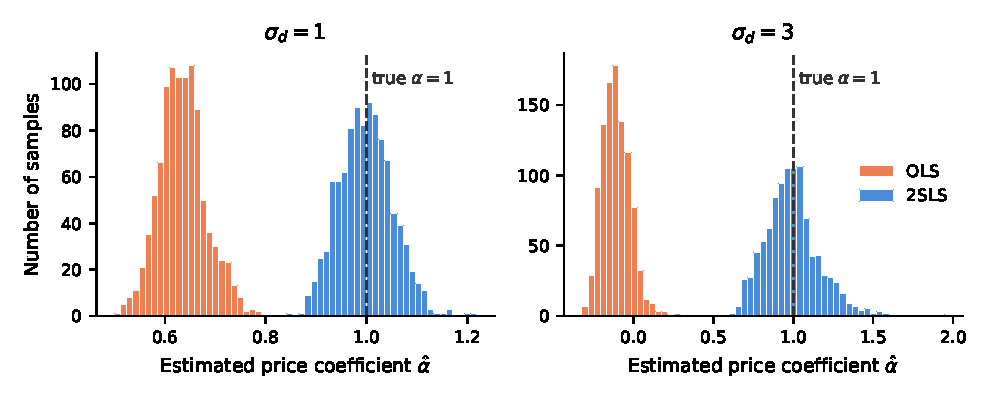
\includegraphics[width=\linewidth]{figures/ch07/mc_logit_ols_iv.pdf}
\caption{Sampling distributions of the estimated price coefficient $\hat\alpha$ in 1,000 samples of 500 duopoly
markets, for the design of \citet[Section~8]{Berry1994}. Left: $\sigma_d = 1$. Right: $\sigma_d = 3$. The dashed line
marks the true value $\alpha = 1$. OLS means are 0.635 and $-0.109$, and 2SLS means are 0.999 and 0.992. Source:
\texttt{figures/ch07/src/mc\_logit\_iv.py}.}
\label{fig:07-mc-ols-iv}
\end{figure}

\casehead{Results}
\Cref{tab:07-mc-logit} places Berry's numbers next to ours, and \cref{fig:07-mc-ols-iv} shows the sampling
distributions of $\hat\alpha$. The qualitative findings replicate. OLS underestimates the price coefficient in every
sample, while 2SLS is centered on the truth (means 1.010 and 1.002, against Berry's 0.995 and 0.979). The OLS bias is
much larger when $\xi$ explains more of mean utility. With $\sigma_d = 1$, OLS implies inelastic demand for 5.3
percent of products, and 99 of our 100 samples contain at least one such product. Berry notes that the OLS estimate
then makes firms appear to price ``on an inelastic portion of their demand curves.'' With $\sigma_d = 3$, he finds
that OLS ``sometimes'' gives $\hat\alpha < 0$. In our replication this happens in 90 of 100 samples.

Our OLS bias is larger than Berry's (mean $\hat\alpha$ of 0.638 and $-0.120$, against 0.726 and 0.181). The 2SLS
results agree closely, so the equilibrium computation and the estimators are unlikely sources of the gap. Berry does
not report every detail, such as the treatment of markets with extreme shares or how his standard errors were
computed. We report our numbers as they come out. The qualitative conclusions do not depend on the gap.

\Cref{prop:07-ols-bias} accounts for the OLS numbers. In a large simulated sample with $\sigma_d = 1$ (20,000 markets),
the projection of price on $x_j$ has slope $\Gamma = 1.847$. With $\hat\alpha_{OLS} = 0.638$ the bias in the price
coefficient is $b = 0.362$, and \eqref{eq:07-ols-bias} predicts $\plim\hat\beta_{x} = 2 - 1.847 \times 0.362 = 1.33$.
The replication mean is 1.335. The bias grows with $\sigma_d$ because the covariance between price and the error
$\sigma_d\xi_j$ scales with $\sigma_d$ twice. It scales once directly, and once through the markup, since by
\eqref{eq:07-dp-dxi} each unit of $\xi_j$ moves price by $\frac{\sigma_d s_j}{\alpha}$. The exogenous price variation
from $w_j$ and $\omega_j$ does not grow with $\sigma_d$.

The experiment also shows which instrument does the work. With $\sigma_d = 1$, the cost shifter alone gives a median
first-stage $F$ of 162. The rival's characteristic alone gives a median $F$ of 1.0, and 2SLS with it alone has a
standard deviation of 1.12 across samples. It is weak because $x$ raises cost as well as utility. In the large sample a
unit increase in $x_j$ raises marginal cost by 1.69 and price by 1.85, so the net mean utility $\beta_0 + \beta_x x_j +
\sigma_d\xi_j - \alpha p_j$ rises by only 0.15. A rival with a higher $x$ is barely more attractive.

\begin{table}[htbp]
\centering
\caption{Rival characteristics as the only instrument: duopoly versus many products.}
\label{tab:07-mc-weak}
\footnotesize
\setlength{\tabcolsep}{4.5pt}
\begin{tabular}{rrccccccc}
\toprule
$J$ & $T$ & Mean $s_0$ & s.d.\ of markups & Median $F$ & \multicolumn{2}{c}{2SLS with $z^{\mathrm{riv}}$} &
2SLS with $w$ & OLS \\
\cmidrule(lr){6-7}
 & & & & & median $\hat\alpha$ & IQR & median $\hat\alpha$ & median $\hat\alpha$ \\
\midrule
2 & 500 & 0.280 & 0.898 & 40.9 & 1.008 & [0.930, 1.082] & 1.000 & 0.483 \\
5 & 200 & 0.062 & 0.520 & 13.3 & 1.024 & [0.852, 1.201] & 1.003 & 0.534 \\
10 & 100 & 0.015 & 0.308 & 1.8 & 0.895 & [0.575, 1.346] & 0.991 & 0.557 \\
25 & 40 & 0.003 & 0.147 & 0.5 & 0.763 & [0.180, 1.369] & 0.999 & 0.578 \\
50 & 20 & 0.001 & 0.085 & 0.4 & 0.538 & [$-0.134$, 1.228] & 1.003 & 0.581 \\
\bottomrule
\end{tabular}
\par\smallskip
\parbox{\linewidth}{\footnotesize Notes: Design of \eqref{eq:07-mc-design} with $\sigma_d = 1$ and $\gamma_x = 0$, so
that $x$ does not enter marginal cost. Each sample has $N = 1{,}000$ products split into $T = \frac{1{,}000}{J}$
markets of $J$ single-product firms, with 200 samples per row. The instrument $z^{\mathrm{riv}}_{j}$ is the sum of $x$ over
the other products in the market. IQR is the interquartile range across samples. The markup standard deviation is computed within each sample and averaged. Source:
\texttt{figures/ch07/src/mc\_logit\_iv.py}.}
\end{table}

\Cref{tab:07-mc-weak} uses the same machinery to show the many-products problem of \citet{Armstrong2016}. We set
$\gamma_x = 0$, so that a rival's characteristic shifts its appeal one for one, and vary the number of products per
market $J$ with 1,000 observations in total. In duopoly the rival characteristic is a strong instrument (median $F$ of
40.9). As $J$ grows, shares shrink, markups converge to $\frac{1}{\alpha} = 1$, and their standard deviation falls from
0.90 to 0.08. The first-stage $F$ falls below 2 at $J = 10$, and the 2SLS estimate drifts toward OLS with exploding
dispersion. The cost shifter is unaffected, with medians within 0.01 of the truth in every row.

\section{The supply side: Bertrand pricing with logit demand}\label{sec:07-supply}

Combined with a model of pricing, demand estimates give markups and marginal costs and let us predict prices after
a merger or a tax. With logit demand almost everything has a closed form: markups, best responses, the equilibrium
aggregate, and pass-through. \Cref{ch:diffprod} proves these results for any ownership structure, and we restate them
here with cross-references. We then use the markups to recover marginal costs, test conduct and simulate mergers. The
closed forms make the logit a benchmark for numerical code, and they expose supply-side restrictions that mirror the
logit's restrictions on substitution. Firms set prices simultaneously, marginal costs are constant, every firm knows
all primitives (including every $\xi_j$), and the market has $M$ consumers. We drop the market index $t$. The general
theory is in \cref{ch:diffprod} and \cref{ch:blp}.

\subsection{Single-product firms}\label{sec:07-bertrand-single}

Firm $j$ sells product $j$ and earns $\pi_j = M(p_j - mc_j)s_j(\boldsymbol p)$. Write $m_j = p_j - mc_j$ for its dollar
markup.

\begin{proposition}[Logit markups with single-product firms]\label{prop:07-logit-markup}
Under logit demand, a single-product firm's best response to any vector of rival prices is characterized by its
first-order condition (\cref{prop:04-logit-br}). By \cref{prop:04-logit-markup}, in any Bertrand-Nash equilibrium
\begin{equation}\label{eq:07-logit-markup}
  p_j - mc_j = \frac{1}{\alpha(1 - s_j)}, \qquad \frac{p_j - mc_j}{p_j} = \frac{1}{\alpha p_j(1 - s_j)} =
  \frac{1}{\varepsilon_j}.
\end{equation}
Markups exceed $\frac{1}{\alpha}$ and depend on product characteristics, prices and costs only through the product's
own market share.
\end{proposition}

The markup is the single-product case of \cref{prop:04-logit-markup}. With $\frac{\partial s_j}{\partial p_j} =
-\alpha s_j(1 - s_j)$ from \cref{prop:07-logit-derivs}, the derivative of profit factors as $M s_j[1 - \alpha m_j(1 -
s_j)]$. The bracket falls strictly once $m_j > 0$ and crosses zero exactly once, and \cref{ch:diffprod} shows that the
crossing is the global maximizer. Dividing the markup by $p_j$ and using $\varepsilon_j = \alpha p_j(1 - s_j)$ gives
the Lerner form.

Two products with the same share therefore have the same dollar markup, whatever their characteristics or costs.
With small shares every markup is close to $\frac{1}{\alpha}$, so Lerner indices are roughly inversely proportional to
price. This is the supply-side image of an own elasticity that rises almost proportionally with price
(\cref{sec:07-iia}), and \cref{sec:07-limits} contrasts it with random coefficient estimates.

The first-order condition is implicit, because $s_j$ depends on $p_j$. It has a closed-form solution in terms of the
\emph{Lambert $W$ function}, defined as the inverse of $u \mapsto ue^u$ on $[0, \infty)$, so that $W(z)e^{W(z)} = z$
for $z \ge 0$ \citep{CorlessEtAl1996}. $W$ is increasing, $W(0) = 0$, and $W'(z) = \frac{W(z)}{z(1 + W(z))}$ for $z >
0$. Define
\begin{equation*}
  v_j = x_j\beta + \xi_j - \alpha\,mc_j, \qquad D_{-j} = 1 + \sum_{l \neq j} e^{\delta_l}.
\end{equation*}
The first is the mean utility product $j$ would have if priced at marginal cost, so $\delta_j = v_j - \alpha m_j$. The
second depends only on rivals' prices. Then $1 - s_j = \frac{D_{-j}}{D_{-j} + e^{\delta_j}}$, and the first-order
condition $\alpha m_j (1 - s_j) = 1$ becomes
\begin{align*}
  \alpha m_j D_{-j} &= D_{-j} + e^{v_j - \alpha m_j} \\
  (\alpha m_j - 1) D_{-j} &= e^{v_j - \alpha m_j} \\
  (\alpha m_j - 1)e^{\alpha m_j - 1} &= \frac{e^{v_j - 1}}{D_{-j}} .
\end{align*}
The last line multiplies both sides by $\frac{e^{\alpha m_j - 1}}{D_{-j}}$. It has the form $ue^u = z$ with $u = \alpha
m_j - 1$, so $u = W(z)$ and
\begin{equation}\label{eq:07-br-lambert}
  BR_j(\boldsymbol p_{-j}) = mc_j + \frac{1}{\alpha}\Bigl[1 + W\Bigl(\frac{e^{v_j - 1}}{D_{-j}}\Bigr)\Bigr].
\end{equation}
This is \eqref{eq:04-logit-br} of \cref{ch:diffprod}, where $D_{-j}$ is written $\Phi_{-j}$. The best response lies
between two bounds. As rival prices fall without limit, $D_{-j} \to \infty$ and the best
response falls to $mc_j + \frac{1}{\alpha}$. As rival prices rise without limit, $D_{-j} \to 1$ and the best response
rises to the monopoly price $mc_j + \frac{1}{\alpha}[1 + W(e^{v_j - 1})]$.

The slope of the best response follows from the chain rule. Since $\frac{\partial D_{-j}}{\partial p_l} = -\alpha
e^{\delta_l}$ for $l \neq j$, the argument $z = \frac{e^{v_j - 1}}{D_{-j}}$ satisfies $\frac{\partial z}{\partial p_l} =
\frac{\alpha z e^{\delta_l}}{D_{-j}}$, and
\begin{equation*}
  \frac{\partial BR_j}{\partial p_l} = \frac{1}{\alpha}W'(z)\frac{\partial z}{\partial p_l}
  = \frac{W(z)}{1 + W(z)}\,\frac{e^{\delta_l}}{D_{-j}} .
\end{equation*}
At the best response, $1 + W(z) = \alpha m_j = \frac{1}{1 - s_j}$, so $\frac{W(z)}{1 + W(z)} = s_j$. Also
$\frac{e^{\delta_l}}{D_{-j}} = \frac{s_l}{1 - s_j}$. Hence
\begin{equation}\label{eq:07-br-slope}
  \frac{\partial BR_j}{\partial p_l} = \frac{s_j s_l}{1 - s_j} > 0, \qquad
  \sum_{l \neq j}\frac{\partial BR_j}{\partial p_l} = s_j\,\frac{1 - s_j - s_0}{1 - s_j} < s_j .
\end{equation}
Prices are \emph{strategic complements}: a rival's price increase raises the firm's best response. The response is less
than one for one in total. The share at the best response is bounded by its monopoly value $\bar s_j =
\frac{W(e^{v_j - 1})}{1 + W(e^{v_j - 1})} < 1$, because $z \le e^{v_j - 1}$. The row sums of the Jacobian of the
best-response map are therefore below $\max_j \bar s_j < 1$ at every price vector. \Cref{prop:04-logit-br} uses this
bound to show that the map is a contraction, so the equilibrium is unique and best-response iteration converges to it
from any starting point.

\begin{figure}[htbp]
\centering
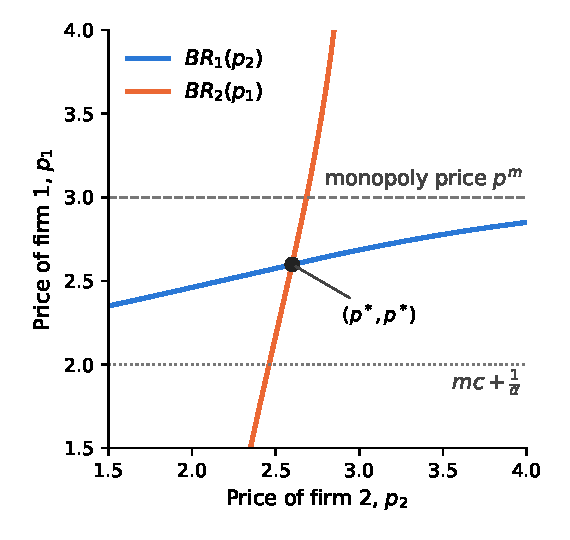
\includegraphics[width=0.52\linewidth]{figures/ch07/logit_best_response.pdf}
\caption{Best responses in a symmetric logit duopoly with an outside good, from \eqref{eq:07-br-lambert}. Both
products have $x_j\beta + \xi_j = 3$ and $mc_j = 1$, and $\alpha = 1$. The horizontal lines bound $BR_1$: it
approaches $mc + \frac{1}{\alpha} = 2$ as $p_2$ falls and the monopoly price $p^m = 3$ as $p_2$ rises. The unique
equilibrium is $p^* = 2.599$ with shares $s_j = 0.375$, where the slope of each best response is $\frac{s_j^2}{1 - s_j}
= 0.224$. Source: \texttt{figures/ch07/src/logit\_best\_response.py}.}
\label{fig:07-best-response}
\end{figure}

\Cref{fig:07-best-response} draws the two best responses of a symmetric duopoly. Each is increasing and flat, and they
cross once. At the equilibrium the markup is $p^* - mc = 1.599$, which equals $\frac{1}{\alpha(1 - s_j)} =
\frac{1}{0.625}$ up to rounding.

\subsection{Multi-product firms}\label{sec:07-bertrand-multi}

Now firm $f$ owns the set $\mathcal{J}_f$ and maximizes $\pi_f = M\sum_{k \in \mathcal{J}_f}(p_k - mc_k)s_k(\boldsymbol
p)$. The first-order condition for $j \in \mathcal{J}_f$ is
\begin{equation}\label{eq:07-multi-foc}
  s_j + \sum_{k \in \mathcal{J}_f}(p_k - mc_k)\frac{\partial s_k}{\partial p_j} = 0 .
\end{equation}
Stacking over all products with the ownership matrix $\Omega$ and the derivative matrix $\Delta$, $\Delta_{jk} =
\frac{\partial s_j}{\partial p_k}$, gives
\begin{equation}\label{eq:07-multi-foc-matrix}
  \boldsymbol s + (\Omega \odot \Delta)^\top(\boldsymbol p - \boldsymbol{mc}) = 0, \qquad
  \boldsymbol p - \boldsymbol{mc} = -\bigl[(\Omega \odot \Delta)^\top\bigr]^{-1}\boldsymbol s,
\end{equation}
as in \cref{ch:diffprod}. Because $\Omega$ is symmetric, $(\Omega \odot \Delta)^\top = \Omega \odot \Delta^\top$. With
logit demand the matrix inversion is unnecessary.

\begin{proposition}[Common markups with multi-product firms]\label{prop:07-logit-multi}
By \cref{prop:04-logit-markup}, under logit demand every solution of the first-order conditions
\eqref{eq:07-multi-foc}, and hence every Bertrand-Nash equilibrium, gives every product of firm $f$ the same dollar
markup
\begin{equation}\label{eq:07-logit-multi}
  m_f = \frac{1}{\alpha(1 - S_f)}, \qquad S_f = \sum_{k \in \mathcal{J}_f} s_k .
\end{equation}
\end{proposition}

The proof in \cref{ch:diffprod} substitutes the logit derivatives into \eqref{eq:07-multi-foc}. This gives $m_j =
\frac{1}{\alpha} + \sum_{k \in \mathcal{J}_f} s_k m_k$ for every $j \in \mathcal{J}_f$, and the right side does not
depend on $j$.

The common markup has a clean interpretation. Substitute $\frac{\partial s_j}{\partial p_j} = -\alpha s_j(1 - s_j)$
and $\frac{\partial s_k}{\partial p_j} = \alpha s_j s_k$ into \eqref{eq:07-multi-foc} and divide by $\alpha s_j(1 -
s_j)$:
\begin{equation}\label{eq:07-recapture}
  m_j = \frac{1}{\alpha(1 - s_j)} + \sum_{k \in \mathcal{J}_f,\, k \neq j} D_{jk}\, m_k, \qquad D_{jk} = \frac{s_k}{1 -
  s_j}.
\end{equation}
The first term is the single-product markup. The second is the value of the sales that a price increase on $j$
diverts to the firm's other products, where $D_{jk}$ is the logit diversion ratio (\cref{sec:07-logit-elasticities}).
A multi-product firm internalizes this recapture, so it prices above the single-product level. In the logit,
diversion is proportional to shares, so recapture depends on the firm's total share and on nothing else. The second
term of \eqref{eq:07-recapture} is the upward pricing pressure that a merger creates (\cref{ch:mergers}). Because
markups are common in dollars, the firm's cheaper products carry the higher percentage markups.

The best response of a multi-product firm also has a closed form. Holding rival prices fixed, every stationary point
of $\pi_f$ has common markups by \cref{prop:07-logit-multi}. Let $E_f = \sum_{k \in \mathcal{J}_f} e^{v_k}$ and $D_{-f} = 1 +
\sum_{l \notin \mathcal{J}_f} e^{\delta_l}$. With a common markup, $S_f = \frac{E_f e^{-\alpha m_f}}{D_{-f} + E_f
e^{-\alpha m_f}}$, and the steps that led to \eqref{eq:07-br-lambert} give
\begin{equation}\label{eq:07-br-multi}
  m_f^{BR} = \frac{1}{\alpha}\Bigl[1 + W\Bigl(\frac{E_f e^{-1}}{D_{-f}}\Bigr)\Bigr], \qquad
  p_k = mc_k + m_f^{BR} \text{ for } k \in \mathcal{J}_f .
\end{equation}
This is \eqref{eq:04-logit-br-multi} of \cref{ch:diffprod}. The firm's products enter only through the sum $E_f$, a
property that the uniqueness proof of \cref{thm:04-logit-unique} exploits.

\Cref{ex:04-logit25} solves both pricing games in one market with 25 products, five owners and $\alpha = 2$, and
\cref{tab:04-logit25} reports the results. With single-product firms, markups range from 0.502 to 0.566, all close to
$\frac{1}{\alpha} = 0.5$. Under the actual ownership each owner has one markup, equal to $\frac{1}{\alpha(1 - S_f)}$.
It ranges from 0.524 for the owner with the smallest combined share to 0.670 for the owner with the largest. Every
price rises, the outside share rises from 0.137 to 0.160, and total profit rises by about 14 percent. \Cref{app:problems}
works through the full problem.

\subsection{Existence and uniqueness of equilibrium}\label{sec:07-uniqueness}

Counterfactuals need a unique equilibrium. Without it, a merger simulation does not tell us which of several
post-merger price vectors to expect. Uniqueness can fail in general pricing games, and \cref{ch:diffprod} discusses the
conditions of \citet{CaplinNalebuff1991} for single-product firms. For the logit, uniqueness holds for any ownership
structure. The single-product case follows from Caplin and Nalebuff and from the contraction argument after
\eqref{eq:07-br-slope}. The multi-product case is due to \citet[Theorem~7, p.~279]{KonovalovSandor2010} and
\citet{NockeSchutz2018}.
In an \emph{aggregative game} each firm's profit depends on its rivals' prices only through one aggregator, and
consumer surplus is a monotone function of it \citep[p.~229, n.~127]{AskerNocke2021}. The logit pricing game is
aggregative, and its aggregator is the inclusive sum $\Lambda = 1 + \sum_k e^{\delta_k}$, which \cref{ch:diffprod}
writes as $\Phi$.

\begin{proposition}[Existence and uniqueness]\label{prop:07-logit-unique}
With logit demand, constant marginal costs and any partition of the products among firms, the Bertrand-Nash pricing
game has exactly one equilibrium. This is \cref{thm:04-logit-unique}.
\end{proposition}

The proof of \cref{thm:04-logit-unique} reduces the equilibrium to one equation in one unknown, the aggregate
$\Lambda$. Each firm sets the common markup of \cref{prop:07-logit-multi}, so its combined share is $S_f = \frac{E_f
e^{-\alpha m_f}}{\Lambda}$, with $E_f$ as in \eqref{eq:07-br-multi}. Substituting $\alpha m_f = \frac{1}{1 - S_f}$
gives
\begin{equation}\label{eq:07-share-aggregate}
  S_f\, e^{\frac{1}{1 - S_f}} = \frac{E_f}{\Lambda} .
\end{equation}
The left side rises strictly from 0 to $+\infty$ as $S_f$ rises from 0 to 1. Each firm's share is therefore a
continuous and strictly decreasing function $S_f(\Lambda)$ of the aggregate. The inside shares and the outside share
$\frac{1}{\Lambda}$ add up to one, so the equilibrium aggregate solves
\begin{equation}\label{eq:07-psi}
  \Psi(\Lambda) \equiv \sum_f S_f(\Lambda) + \frac{1}{\Lambda} = 1 .
\end{equation}
The function $\Psi$ is strictly decreasing, exceeds one at $\Lambda = 1$ and tends to zero as $\Lambda \to \infty$.
It has exactly one root $\Lambda^* > 1$, and the root pins down every share, markup and price.

The characterization doubles as an algorithm: solve \eqref{eq:07-psi} by bisection and read off shares, markups and
prices. Best-response iteration with \eqref{eq:07-br-multi}, the markup fixed point $\boldsymbol p \leftarrow
\boldsymbol{mc} + \frac{1}{\alpha(1 - S_f(\boldsymbol p))}$, and Newton's method are common alternatives. In the
market of \cref{ex:04-logit25}, $\Lambda^* = 7.314$ with single-product firms and $6.246$ with multi-product firms,
equal to $\frac{1}{s_0}$ in each case (\cref{ex:04-logit25-unique}). With non-logit demand uniqueness is not
guaranteed, and restarting the solver from many points is the practical check (\cref{ch:blp}).

\subsection{Pass-through}\label{sec:07-passthrough}

The \emph{pass-through rate} $\rho = \frac{\dd p}{\dd mc}$ measures how much of a cost change reaches the price
(\cref{ch:theory}). It governs the incidence of taxes, the effect of exchange rates on import prices, and the price
effect of merger efficiencies.

\begin{proposition}[Logit pass-through]\label{prop:07-logit-passthrough}
Hold rivals' prices fixed. By parts (i) and (iii) of \cref{prop:04-passthrough}, the following hold.
\begin{enumerate}[label=(\roman*)]
  \item A single-product firm passes through $\rho_j = \frac{\dd p_j}{\dd mc_j} = 1 - s_j$ of an increase in its
    marginal cost.
  \item A multi-product firm facing the same increase in the marginal cost of all its products raises all its prices by
    $\rho_f = 1 - S_f$ per unit of cost.
\end{enumerate}
In both cases pass-through is below one and falls with the firm's share.
\end{proposition}

The proof in \cref{ch:diffprod} differentiates the markup condition $\alpha m_f(1 - S_f) = 1$. A common cost increase
$\dd mc$ lowers the firm's combined share, and the common markup falls by $S_f\,\dd mc$, so each price rises by $(1 -
S_f)\,\dd mc$. A single-product firm is the case $S_f = s_j$.

Pass-through below one is the logit instance of a general result for log-concave demand. For a single-product firm
with demand $q(p)$ at fixed rival prices, \eqref{eq:02-pt-logcurv} gives
\begin{equation*}
  \rho = \frac{\dd p}{\dd mc} = \frac{1}{2 - \frac{q q''}{(q')^2}} ,
\end{equation*}
and $\rho < 1$ exactly when demand is log-concave at the optimum (\cref{cor:02-bulow-pfleiderer}).
\citet{BulowPfleiderer1983} write the same pass-through rate in terms of the demand elasticity and its slope, as
restated by \citet[p.~18 of the 2008 working paper]{FarrellShapiro2010}. \citet{WeylFabinger2013} develop pass-through
as a general tool for incidence under imperfect competition. Holding rivals' prices fixed, logit demand is log-concave
in own price:
\begin{equation*}
  \frac{\dd \ln s_j}{\dd p_j} = -\alpha(1 - s_j), \qquad \frac{\dd^2 \ln s_j}{\dd p_j^2} = \alpha\frac{\dd s_j}{\dd p_j}
  = -\alpha^2 s_j(1 - s_j) < 0 .
\end{equation*}
With $q = s_j$, $q' = -\alpha s_j(1 - s_j)$ and $q'' = \alpha^2 s_j(1 - s_j)(1 - 2s_j)$, the ratio $\frac{q
q''}{(q')^2}$ equals $\frac{1 - 2s_j}{1 - s_j}$, and the general formula returns $\rho_j = 1 - s_j$.
In the market of \cref{ex:04-logit25} the largest owner has $S_f = 0.2536$, and a numerical derivative of
\eqref{eq:07-br-multi} gives pass-through 0.7464, equal to $1 - S_f$. The proposition holds rivals' prices fixed.
When a cost shock hits all firms, rivals raise their prices as well. By strategic complementarity
\eqref{eq:07-br-slope}, equilibrium pass-through then exceeds $1 - s_j$ (\cref{cor:04-passthrough-eq}).

\begin{figure}[htbp]
\centering
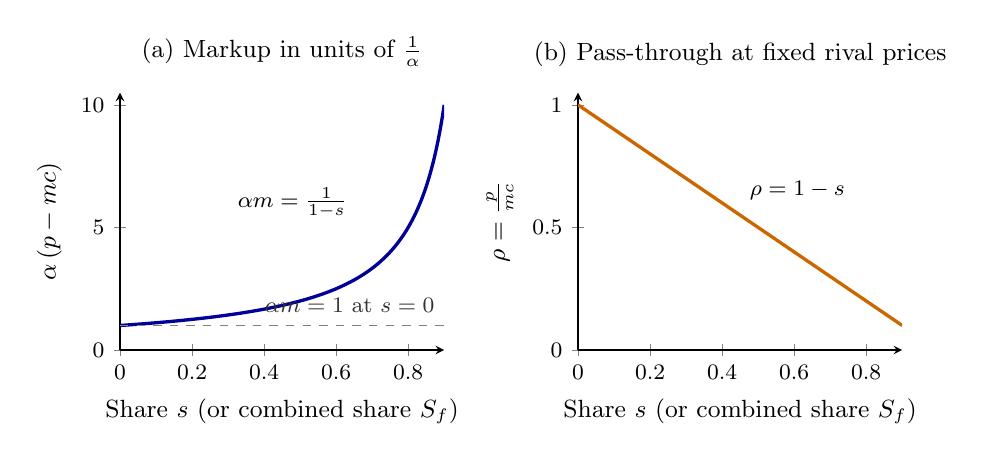
\begin{tikzpicture}
\begin{axis}[
  name=leftax, width=0.47\linewidth, height=0.40\linewidth,
  xmin=0, xmax=0.9, ymin=0, ymax=10.5,
  xlabel={Share $s$ (or combined share $S_f$)}, ylabel={$\alpha\,(p - mc)$},
  title={(a) Markup in units of $\frac{1}{\alpha}$},
  title style={font=\small}, label style={font=\small}, tick label style={font=\footnotesize},
  domain=0:0.9, samples=200, axis lines=left]
  \addplot[very thick, blue!60!black] {1/(1-x)};
  \node[font=\footnotesize, anchor=west] at (axis cs:0.30,6.0) {$\alpha m = \frac{1}{1 - s}$};
  \addplot[dashed, gray] coordinates {(0,1) (0.9,1)};
  \node[font=\footnotesize, anchor=south east, gray!40!black] at (axis cs:0.90,1.15) {$\alpha m = 1$ at $s = 0$};
\end{axis}
\begin{axis}[
  at={(leftax.east)}, anchor=west, xshift=1.7cm,
  width=0.47\linewidth, height=0.40\linewidth,
  xmin=0, xmax=0.9, ymin=0, ymax=1.05,
  xlabel={Share $s$ (or combined share $S_f$)}, ylabel={$\rho = \frac{\dd p}{\dd mc}$},
  title={(b) Pass-through at fixed rival prices},
  title style={font=\small}, label style={font=\small}, tick label style={font=\footnotesize},
  domain=0:0.9, samples=50, axis lines=left]
  \addplot[very thick, orange!80!black] {1-x};
  \node[font=\footnotesize, anchor=west] at (axis cs:0.45,0.65) {$\rho = 1 - s$};
\end{axis}
\end{tikzpicture}
\caption{Logit markups and pass-through as functions of the firm's share. Panel (a): the dollar markup times $\alpha$,
from \cref{prop:07-logit-markup,prop:07-logit-multi}. Panel (b): the pass-through rate of
\cref{prop:07-logit-passthrough}. For a multi-product firm, read the horizontal axis as $S_f$.}
\label{fig:07-markups}
\end{figure}

\Cref{fig:07-markups} summarizes the two results. Markups rise and pass-through falls with the firm's share, and
nothing else about the product matters. The link to merger analysis is direct. \citet{FarrellShapiro2010} define the
upward pricing pressure on product $j$ after a merger with the owner of $k$ as $D_{jk}m_k$, the second term of
\eqref{eq:07-recapture}. They evaluate it at pre-merger prices and before any credit for cost savings (p.~9 of their
2008 working paper). \citet[p.~231]{AskerNocke2021} state the same definition and read it as the merged firm's
opportunity cost of keeping the price of $j$ at its pre-merger level. It acts like a cost increase on $j$, so to first
order the price of $j$ rises by
$\rho_j D_{jk}m_k = (1 - s_j)\frac{s_k}{1 - s_j}m_k = s_k m_k$ under logit demand. \Cref{ch:mergers} develops this
approximation and its limits.

\subsection{Recovering marginal costs and joint estimation}\label{sec:07-cost-recovery}

Given an estimate $\hat\alpha$ and an assumed ownership structure, the first-order conditions deliver marginal costs
without any cost data. Suppose marginal cost is linear in observed cost shifters $w_{jt}$ and a cost shock
$\omega_{jt}$, $mc_{jt} = w_{jt}\gamma + \omega_{jt}$. By \cref{prop:07-logit-multi},
\begin{equation}\label{eq:07-logit-supply}
  p_{jt} = w_{jt}\gamma + \frac{1}{\alpha(1 - S_{ft})} + \omega_{jt},
  \qquad \widehat{mc}_{jt} = p_{jt} - \frac{1}{\hat\alpha(1 - S_{ft})} .
\end{equation}
With single-product firms ($S_{ft} = s_{jt}$) the first equation is equation (31) of \citet[p.~255]{Berry1994},
whose parameters are $\gamma$ and $\frac{1}{\alpha}$. His general version (equation 29) lets cost depend on output and
writes the markup as $\frac{s_j}{\alpha}\bigl(\frac{\partial s_j}{\partial\delta_j}\bigr)^{-1}$, which covers any demand
model. The
nested logit version is \cref{prop:07-nl-markup}.

There are two ways to estimate $\gamma$. The \emph{two-step} approach regresses $\widehat{mc}_{jt}$ on $w_{jt}$ by
OLS. It is consistent when $\E[w_{jt}^\top\omega_{jt}] = 0$ and $\hat\alpha$ is consistent. Its usual standard errors
are wrong, because the dependent variable is a \emph{generated regressand}. The error in the implied cost is
\begin{equation*}
  \widehat{mc}_{jt} - mc_{jt} = \frac{1}{\alpha(1 - S_{ft})} - \frac{1}{\hat\alpha(1 - S_{ft})} \approx
  \frac{\hat\alpha - \alpha}{\alpha^2(1 - S_{ft})} ,
\end{equation*}
which is nearly common to all products when shares are small, so it loads on the intercept of the cost regression.
The simulated market of \cref{sec:08-worked-logit}, which \cref{app:problems} works through, shows the size of the
effect. A market bootstrap that re-estimates $\alpha$ raises the intercept's standard error there from 0.016 to 0.072,
while the slopes' standard errors barely move. Valid inference uses
such a bootstrap or the sandwich of a stacked GMM problem \citep{Newey1984}. Negative implied costs signal a problem
with the demand estimates or the conduct assumption.

The \emph{joint} approach estimates demand and supply together. Let $\theta = (\beta, \alpha, \gamma)$ and define the
two structural errors
\begin{equation}\label{eq:07-joint-errors}
  \xi_{jt}(\theta) = y_{jt} - x_{jt}\beta + \alpha p_{jt}, \qquad
  \omega_{jt}(\theta) = p_{jt} - \frac{1}{\alpha(1 - S_{ft})} - w_{jt}\gamma .
\end{equation}
With demand instruments $z^d_{jt}$ and supply instruments $z^s_{jt}$, the moment conditions are $\E[z^{d\top}_{jt}
\xi_{jt}(\theta)] = 0$ and $\E[z^{s\top}_{jt}\omega_{jt}(\theta)] = 0$. GMM minimizes $\bar g(\theta)^\top W \bar
g(\theta)$ for the stacked sample moments
\begin{equation}\label{eq:07-joint-gmm}
  \bar g(\theta) = \frac{1}{N}\sum_t\sum_{j \in \mathcal{J}_t}
  \begin{pmatrix} z^{d\top}_{jt}\,\xi_{jt}(\theta) \\ z^{s\top}_{jt}\,\omega_{jt}(\theta) \end{pmatrix} .
\end{equation}
For a given $\alpha$ both errors are linear in $(\beta, \gamma)$, which can be concentrated out, so the search is over
$\alpha$ alone. The markup term is endogenous, because $S_{ft}$ depends on prices and hence on $\omega_{jt}$.
\citet[p.~255]{Berry1994} lists its instruments: excluded demand characteristics, characteristics of other firms, and
market population when markets differ in size.

Joint estimation helps when demand instruments are weak, because the markup term carries information about $\alpha$
if the supply instruments overidentify $\gamma$. It also exploits any correlation between $\xi$ and $\omega$, it is
where conduct enters when conduct is tested, and it gives correct standard errors for $\gamma$. The cost is
robustness. A wrong ownership or conduct assumption contaminates the demand estimates through the shared $\alpha$.
Berry notes that joint estimation ``would take into account the cross-equation restrictions on parameters.''
\Cref{ch:blp} develops joint estimation with random coefficients, where the gains are larger.

\subsection{Testing conduct and ownership with logit demand}\label{sec:07-conduct}

The same first-order conditions can be evaluated under different assumptions about who sets which price. Let a
\emph{pricing coalition} be a set of products whose prices are chosen jointly. By \cref{prop:07-logit-multi}, a
coalition $A$ sets the common markup $\frac{1}{\alpha(1 - S_A)}$, where $S_A$ is its combined share. Implied Lerner
indices under four structures are therefore analytic:
\begin{equation}\label{eq:07-conduct-margins}
  \underbrace{\frac{1}{\alpha p_j(1 - s_j)}}_{\text{single product}}, \qquad
  \underbrace{\frac{1}{\alpha p_j(1 - S_f)}}_{\text{actual ownership}}, \qquad
  \underbrace{\frac{1}{\alpha p_j(1 - S_G)}}_{\text{joint pricing of } G}, \qquad
  \underbrace{\frac{1}{\alpha p_j s_0}}_{\text{monopoly}},
\end{equation}
where $G$ is a group of colluding products, and monopoly uses $1 - \sum_{k \ge 1}s_k = s_0$. Comparing the predicted
margins with observed margins, or with outside information on costs, tests the structures. Only $\hat\alpha$ and the
shares are needed.

\citet[Section~5.3]{Nevo2001} carries out this comparison for cereal, and \cref{tab:07-nevo-margins} reproduces the
logit column of his Table VIII. It uses the price coefficient of column (ix) of \cref{tab:07-nevo-logit}. Because only
shares are needed, the logit margins can include brands outside the 25 in the sample, which the full model cannot
\citep[pp.~332--333]{Nevo2001}.

\begin{table}[htbp]
\centering
\caption{Median price-cost margins in ready-to-eat cereal under alternative pricing structures, logit demand.}
\label{tab:07-nevo-margins}
\footnotesize
\begin{tabular}{lc}
\toprule
 & Logit \\
 & (Table V, column ix) \\
\midrule
Single-product firms & 33.6\% \\
 & (31.8\%--35.6\%) \\
Current ownership of 25 brands & 35.8\% \\
 & (33.9\%--38.0\%) \\
Joint ownership of 25 brands & 41.9\% \\
 & (39.7\%--44.4\%) \\
Current ownership of all brands & 37.2\% \\
 & (35.2\%--39.4\%) \\
Monopoly or perfect price collusion & 54.0\% \\
 & (51.1\%--57.3\%) \\
\bottomrule
\end{tabular}
\par\smallskip
\parbox{\linewidth}{\footnotesize Notes: Source: \citet[Table~VIII, p.~333]{Nevo2001}, logit column. Margins are
$\frac{p - mc}{p}$. Entries are medians over 27,862 brand-city-quarter observations, with 95 percent confidence
intervals for the median in parentheses, based on the asymptotic distribution of the demand estimates. The logit
computation is analytical. \Cref{tab:08-nevo-margins} reproduces the full table, including the random coefficients
column.}
\end{table}

Nevo compares the predictions with crude accounting estimates. The gross retail margin is about 46.0 percent, and the
gap between national brands and private labels gives a lower bound of about 31 percent \citep[pp.~333--334]{Nevo2001}.
His full random coefficients model predicts a median margin of 35.8 percent with single-product firms. It is 42.2
percent (interval 29.1 to 55.8) under current ownership and 72.6 percent (62.2 to 97.2) under joint ownership of the
25 brands (\cref{tab:08-nevo-margins}). Using these intervals, he rejects joint profit maximization by the 25 brands and
cannot reject multi-product Nash pricing. The logit column tells a different story. Joint ownership of the 25 brands
raises the logit margin only from 35.8 to 41.9 percent, against 42.2 to 72.6 percent in the full model. With logit
margins, joint ownership comes closer to the accounting margin than current ownership does, so a logit-based test
could point toward collusion.

The logit understates the effect of joint pricing because of IIA. A coalition's markup depends only on
$\frac{1}{1 - S_G}$. With a market of one serving per person per day the outside share is large, so $S_G$ is far from
one even for 25 brands. Diversion is proportional to shares (\cref{sec:07-iia}), so most of the sales a brand loses go
to the outside good, and merging brands recaptures little. In the random coefficient model cereals are closer
substitutes for each other than for the outside good, so joint pricing recaptures much more. The assumed demand model
shapes the conduct test as much as the data do.

\citet[p.~874]{BerryLevinsohnPakes1995} make the same point for cars. Their IV logit implies that ``all models have
about the same mark-up,'' from \$4,630 for the BMW to \$4,805 for the Chevy Cavalier. Shares measured against all
households are tiny, so markups are close to $\frac{1}{\hat\alpha} = \frac{1}{0.216}$ thousand dollars, about \$4,630.
Differences come only from the number of models a parent firm sells. GM sells the most and has the highest markups,
while BMW has, ``quite counter-intuitively,'' the lowest. If BMW's combined share is negligible,
\eqref{eq:07-logit-multi} and $1 - \frac{4{,}630}{4{,}805} \approx 0.036$ imply that GM's models together sold to
roughly 3.6 percent of households. \Cref{sec:07-limits-markups} translates these dollar markups into Lerner
indices, and the random coefficient markups of \cref{ch:blp} vary far more across models.

Comparing implied margins across ownership structures is an alternative to estimating a conduct parameter
(\cref{ch:conduct}). It sidesteps the problem raised by \citet[p.~227]{Corts1999}, who shows that in a dynamic
oligopoly model the estimated conduct parameter can mismeasure market power severely. \citet{Bresnahan1987} applies
a nested test of this kind with the vertical model (\cref{ch:discrete}).

Logit merger simulation follows directly. \citet[p.~230]{AskerNocke2021} credit \citet{HausmanLeonardZona1994},
\citet{WerdenFroeb1994} and \citet{Nevo2000b} with pioneering \emph{merger simulation}, which has three steps. The
first estimates pre-merger demand. The second recovers pre-merger marginal costs from an assumption on pre-merger
conduct, typically static Bertrand-Nash pricing. The third computes the post-merger equilibrium under assumptions on
post-merger conduct and on merger-related cost savings, holding demand and the product set fixed. Werden and Froeb
carry out these steps with logit demand. The first two steps are then analytic, and the third reduces to one
equation in one unknown.
Estimate $\alpha$, recover marginal
costs from \eqref{eq:07-logit-supply} under the pre-merger ownership, and solve \eqref{eq:07-psi} under the
post-merger ownership. If firms $f$ and $f'$ merge, the merged firm sets one
markup $\frac{1}{\alpha(1 - S_f - S_{f'})}$ at post-merger shares, and rivals respond. Because diversion follows
shares, the predicted dollar price effects depend only on $\hat\alpha$, the ownership structure and the pre-merger
shares (\cref{ch:mergers}). When the size of the cost savings is unknown, the third step can instead find the
smallest savings that leave consumer surplus unchanged \citep[pp.~230--231]{AskerNocke2021}.
